\documentclass[12pt]{article}
\usepackage[papersize={8cm,12cm},margin={.5cm,.5cm}]{geometry}
\usepackage{common}
\begin{document}
\begin{problem}
  \item[4.] 圖(一)為鋰離子(\ch{Li^+})的結構示意圖,其中以不同顏色的球表示中子、電子與質子。關於此粒子的敘述,下列何者正確?
  \begin{figure}[ht]
    \centering
    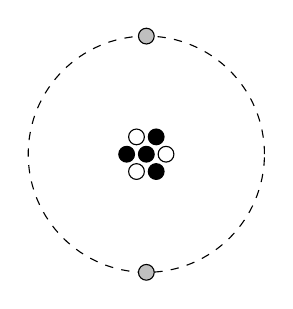
\begin{tikzpicture}
      \draw[dashed] (0,0) circle (1.5cm);
      \draw (-.125,.22) circle (.1cm);
      \draw[fill=black] (.125,.22) circle (.1cm);
      \draw[fill=black] (-.25,0) circle (.1cm);
      \draw[fill=black] (0,0) circle (.1cm);
      \draw (.25,0) circle (.1cm);
      \draw (-.125,-.22) circle (.1cm);
      \draw[fill=black] (.125,-.22) circle (.1cm);
      \draw[fill=black!25] (0,1.5) circle (.1cm);
      \draw[fill=black!25] (0,-1.5) circle (.1cm);
    \end{tikzpicture}
    \caption*{圖(一)}
    \vspace*{-2ex}
  \end{figure}
  \begin{choices}
    \item 原子序為 2
    \item 電子數為 3
    \item 中子數為 4
    \item 質量數為 9
  \end{choices}
\end{problem}
\end{document}
